\documentclass{article}

\usepackage[final]{neurips_2026}

\usepackage[utf8]{inputenc}
\usepackage[T1]{fontenc}
\usepackage{hyperref}
\usepackage{url}
\usepackage{booktabs}
\usepackage{amsfonts}
\usepackage{amsmath}
\usepackage{nicefrac}
\usepackage{microtype}
\usepackage{xcolor}
\usepackage{graphicx}
\graphicspath{{outputs/}}

\title{Estimating the Human Capital Cost of AI Research:\\
NLP Prediction of Research Cost from ArXiv Title and Abstract Text (2022--2026)}

\author{%
  Karamvir Singh \\
  01:198:439 Introduction to Data Science \\
  Instructor: Dr.\ Hongyi Wang \\
  Rutgers University \\
  \texttt{ks1660@rutgers.edu}
}

\begin{document}

\maketitle

\begin{abstract}
This paper addresses the question: \emph{can the human capital cost of AI research be estimated from configurable salary priors and paper metadata, and can NLP predict research cost tier from paper title and abstract text alone?} This paper applies a position-based salary model to 288,368 ArXiv papers across six CS/AI categories, assigning per-author salaries using academic authorship conventions: first author $\approx$ Graduate researcher (\$49K), last author $\approx$ PI/Professor (\$96K), middle authors $\approx$ distribution-weighted mix (\$55K). Per-paper human capital cost averages \$40,239, totalling an estimated \$11.6 billion across all papers, with a measurable growth trend from December 2022 to February 2026. Three NLP classifiers---Naive Bayes with Laplace smoothing, Logistic Regression with L2 regularization, and a neural network MLP---are trained on TF-IDF representations of concatenated paper titles and abstracts to predict cost bucket (Low/Medium/High). The best model (MLP) achieves a weighted F1 of 0.5179 on a held-out test set, demonstrating moderate but statistically meaningful signal between text vocabulary and estimated research cost. K-Means clustering achieves a purity of 0.4363 versus 0.3333 random baseline. All code is available at: \url{https://github.com/KSGH0/CS439\_FINAL\_PROJECT}.
\end{abstract}

\newpage

\section{Introduction}

The cost of AI research is largely invisible. Unlike industrial R\&D, academic research expenditure is rarely reported in aggregate, yet understanding it matters for science policy, funding allocation, and assessing the true resource intensity of AI progress. Human capital---researcher salaries and stipends---constitutes the dominant cost for most academic AI papers.

This project investigates two interconnected questions. First, can the human capital cost of AI research be estimated using configurable salary priors based on academic authorship conventions applied to paper metadata? Second, does the text of a paper's title and abstract encode enough signal about its cost structure that NLP classifiers can predict cost tier above chance?

The dataset consists of 288,368 unique ArXiv papers across six CS/AI subfields (cs.AI, cs.LG, cs.CL, cs.NE, cs.IR, cs.CV) spanning December 1, 2022 to March 5, 2026. Salary estimation uses a position-based model: first authors are assigned graduate researcher salaries (\$49K), last authors PI/Professor salaries (\$96K), and middle authors a distribution-weighted academic mix (\$55K), reflecting standard CS/AI authorship conventions. All salary constants are configurable.

The primary contributions are a position-based salary model applied to 288,368 papers, a monthly cost trend analysis (December 2022--February 2026) showing +14.2\% growth, an NLP pipeline (Naive Bayes, Logistic Regression, MLP) predicting cost tier from paper text with MLP F1 of 0.5179, and unsupervised K-Means validation achieving purity 0.4363 versus 0.3333 random baseline.

\section{Related Work}

\textbf{NLP for document analysis.}
Text classification and feature extraction from scientific documents are well-established tasks covered in~\cite{vanderplalas2023} and~\cite{learningds2023}. This work differs in applying NLP to predict an economic variable---research cost---rather than topic or bibliometric outcomes.

\textbf{Classical NLP classifiers.}
Naive Bayes and Logistic Regression are well-established baselines for high-dimensional text classification~\cite{princetondml, vanderplalas2023, mckinney2022}. All three models in this project are coded from first principles, with the MLP serving as a non-linear comparison point~\cite{princetondml}.

\section{Dataset \& Exploratory Analysis}

\subsection{Dataset}

The dataset draws from six ArXiv JSONL files sourced from the ArXiv AI Research Papers Dataset~\cite{haddii2024} (Kaggle, CC BY 4.0), collecting 417,331 raw paper records covering categories cs.AI, cs.LG, cs.CL, cs.NE, cs.IR, and cs.CV. After deduplication, 288,368 unique papers remain spanning December 1, 2022 to March 5, 2026. Each record provides title, abstract, author list, primary category, and publication date. All 288,368 papers are used for both cost computation and NLP training.

\subsection{Author Distribution with Gaussian KDE}

Figure~\ref{fig:kde} shows the author-per-paper distribution using a Gaussian KDE with bandwidth chosen by Silverman's rule ($h = 1.06\,\hat{\sigma}\,n^{-1/5}$). The distribution is right-skewed with mean 5.16, median 4, and standard deviation 9.26 (heavy right tail from large collaborative projects), reflecting the collaborative nature of modern AI research~\cite{learningds2023}.

\begin{figure}[h]
    \centering
    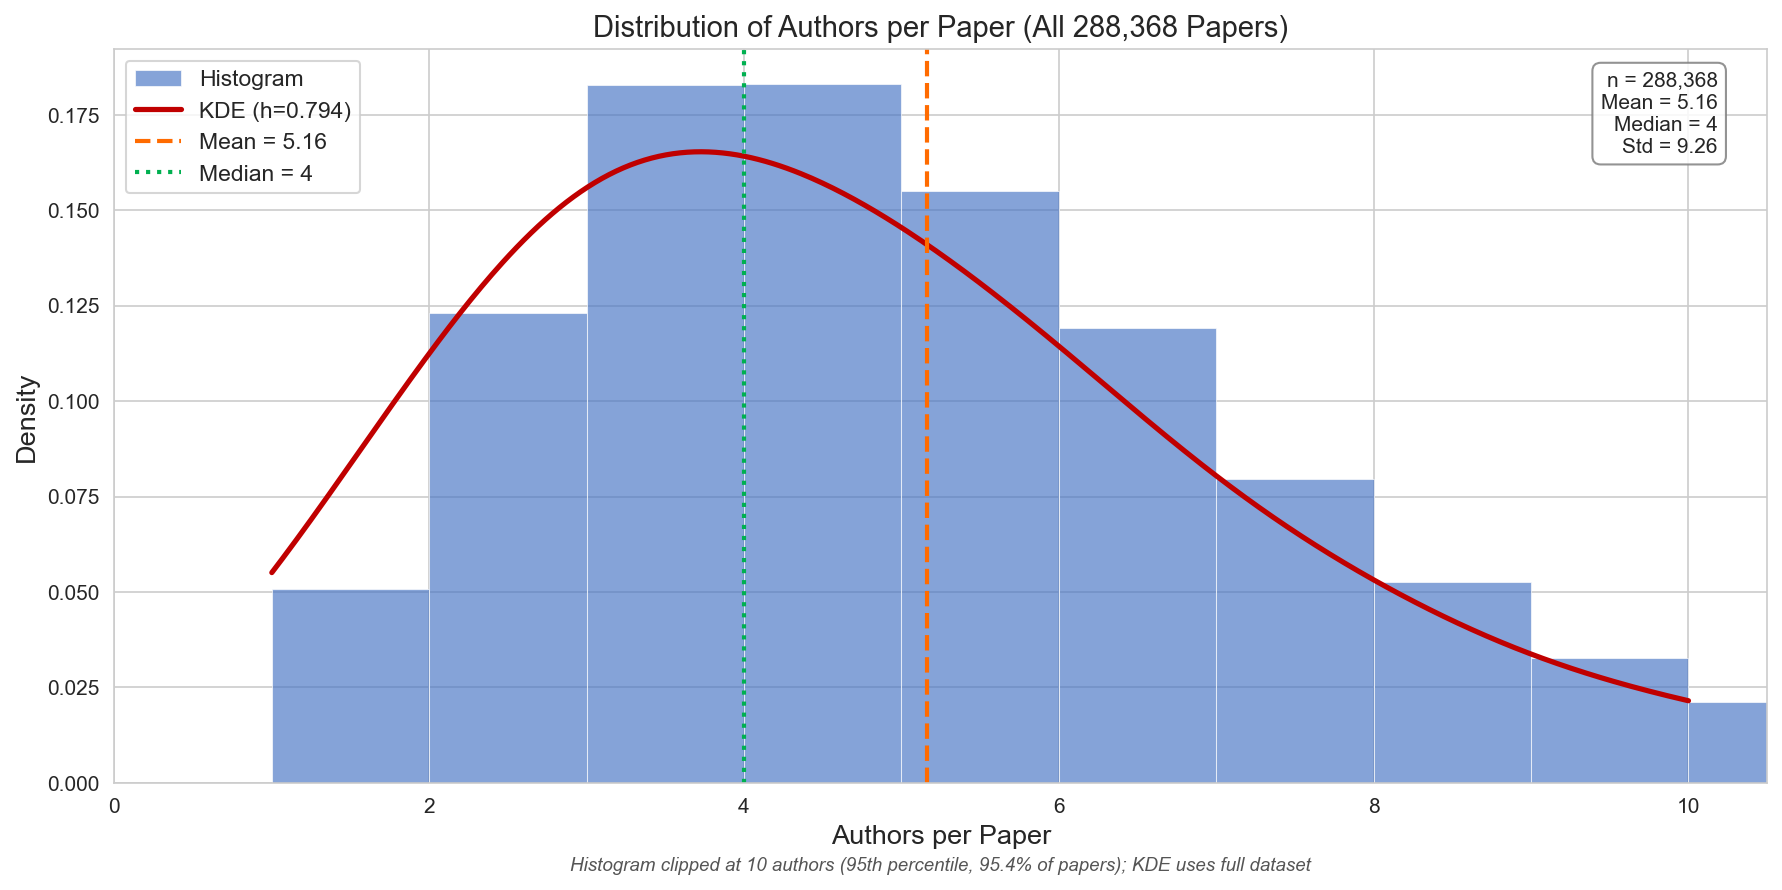
\includegraphics[width=0.85\textwidth]{fig_authors_histogram.png}
    \caption{Distribution of authors per paper (full 288,368-paper dataset) with histogram and Gaussian KDE. Mean = 5.16, median = 4, std = 9.26. The long right tail reflects highly collaborative multi-institution projects.}
    \label{fig:kde}
\end{figure}

\subsection{Cost Distribution by Category}

Figure~\ref{fig:cost_box} shows the estimated human capital cost per paper across all six primary ArXiv categories in the dataset. cs.CL papers are most expensive on average while cs.NE is lowest, consistent with their higher and lower mean author counts respectively (6 vs.\ 4 authors per paper).

\begin{figure}[h]
    \centering
    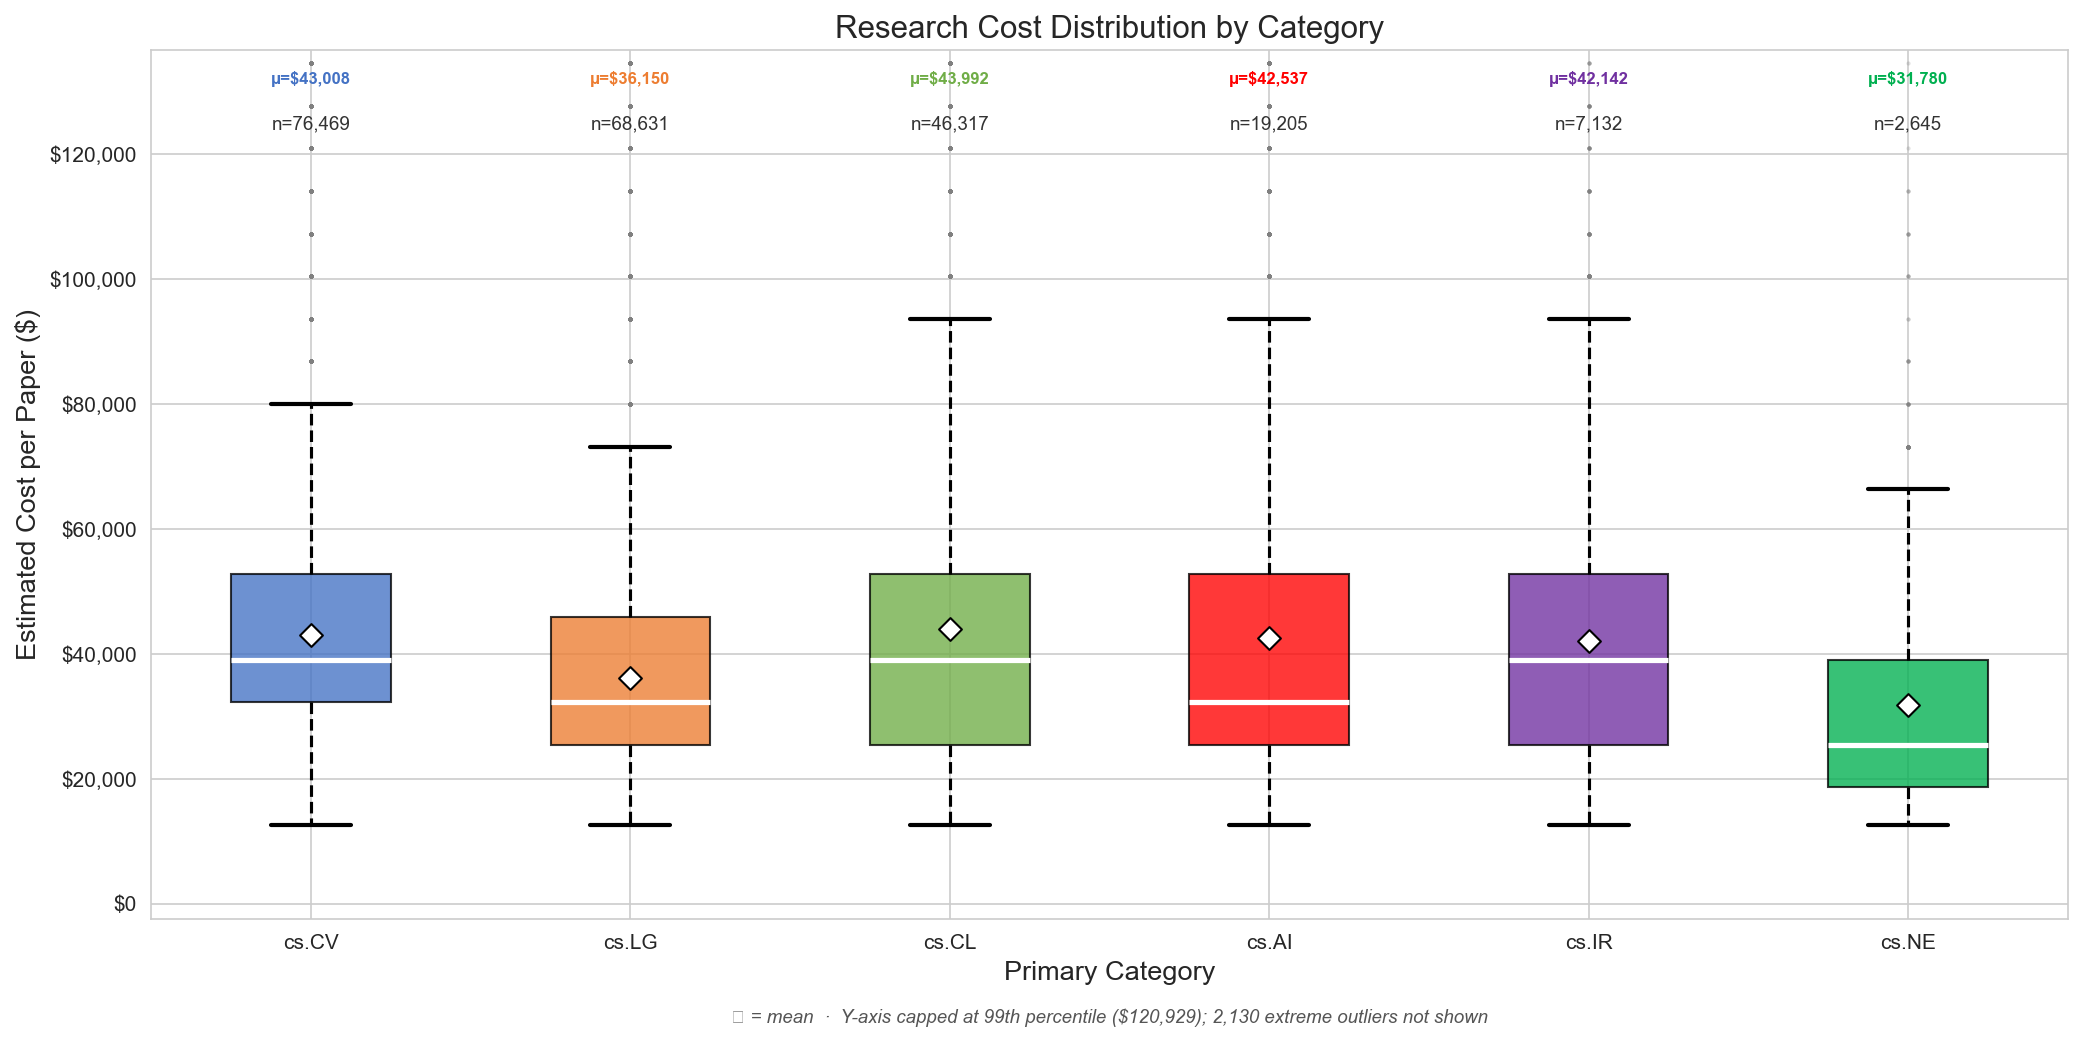
\includegraphics[width=\textwidth]{fig_cost_by_category_box.png}
    \caption{Per-paper estimated human capital cost across the six primary categories. Boxes show IQR; whiskers extend to 1.5$\times$IQR. cs.CL and cs.CV papers tend to involve larger author teams.}
    \label{fig:cost_box}
\end{figure}

\subsection{Temporal Cost Trend}

Figure~\ref{fig:trend} shows mean estimated cost per paper by month from December 2022 to February 2026. March 2026 is excluded as it contains only 5 days of data. The trend is broadly increasing, growing +14.2\% over the period, consistent with general salary growth in AI research roles.

\begin{figure}[h]
    \centering
    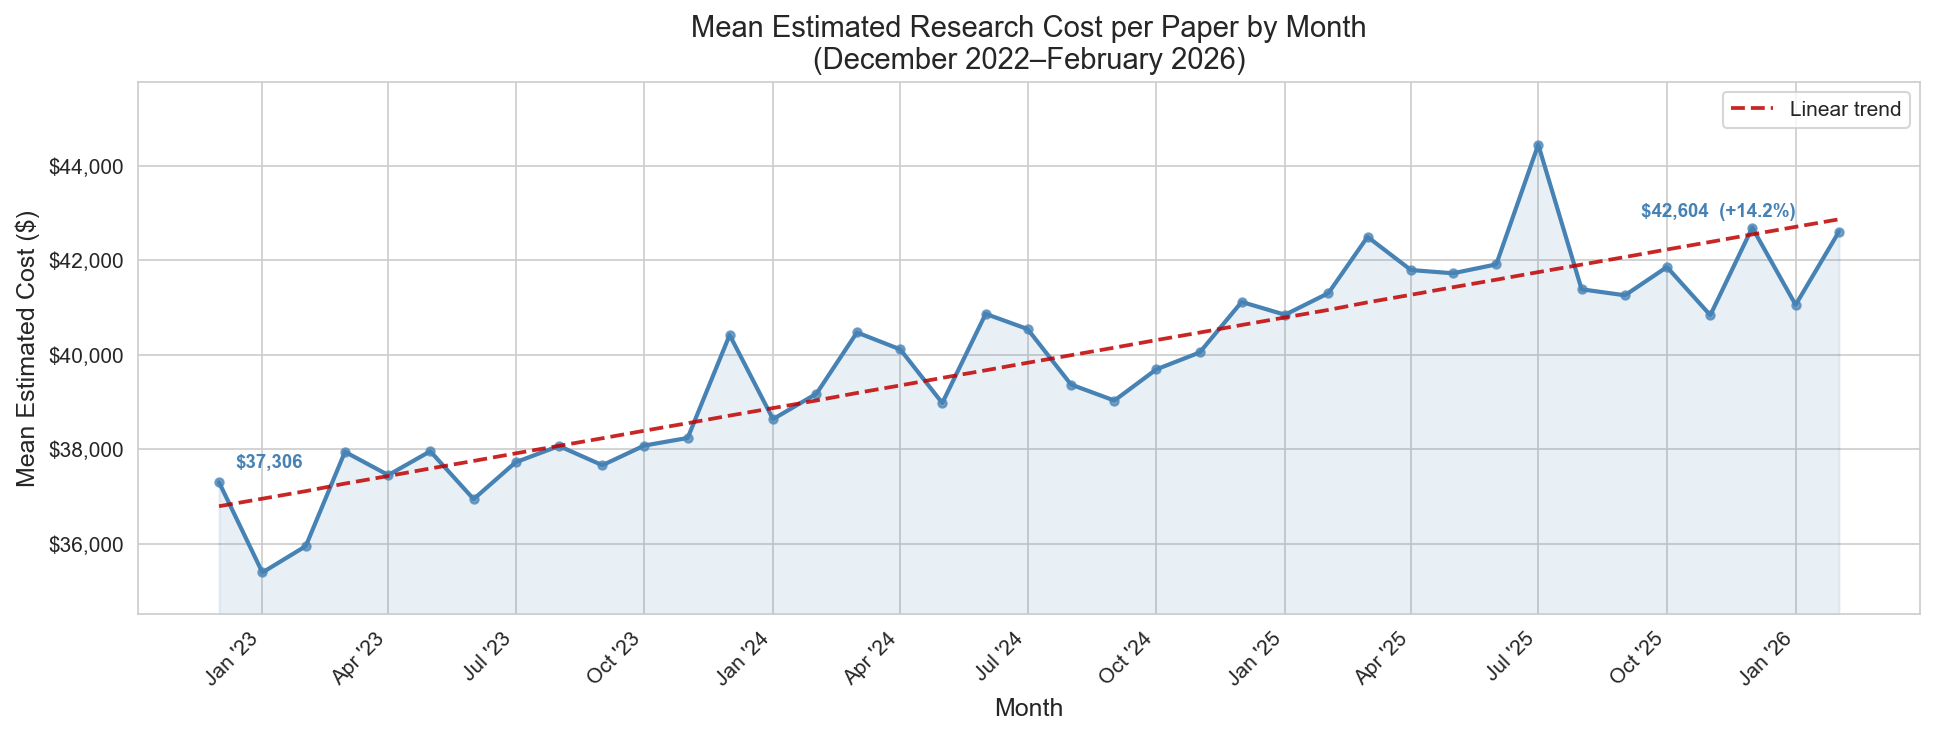
\includegraphics[width=0.85\textwidth]{fig_cost_trend_month.png}
    \caption{Mean estimated human capital cost per paper by month (December 2022--February 2026). March 2026 excluded (5 days only). Monthly grouping eliminates partial-month skew; the upward trend reflects rising researcher salaries and increasing team sizes in modern AI papers.}
    \label{fig:trend}
\end{figure}

\section{Methodology}

\subsection{Position-Based Salary Estimation}

This paper assigns each author an annual salary estimate using a \textbf{position-based role prior} grounded in standard CS/AI authorship conventions. In academic ML papers, authorship order encodes role: the first author typically performs most of the experimental work (graduate researcher), middle authors contribute specific components (mixed seniority), and the last author supervises as PI (professor). This convention is consistent across top venues including NeurIPS, ICML, ICLR, and ACL.

Salary constants reflect commonly reported US academic CS ranges, adjusted by a global salary scaler $\mu$ (default $\mu = 1.0$, all values configurable via the project UI), summarised in Table~\ref{tab:salary_priors}:

\begin{table}[h]
    \centering
    \small
    \caption{Position-based salary priors used to estimate per-author annual compensation.}
    \label{tab:salary_priors}
    \begin{tabular}{llcc}
        \toprule
        \textbf{Author position} & \textbf{Role assumed} & \textbf{Base salary ($\mu$=1)} & \textbf{Notes} \\
        \midrule
        First (pos = 0)       & Graduate researcher  & \$48,500  & PhD + postdoc combined (average) \\
        Last (pos = $n-1$)    & PI/Professor         & \$96,430  & Median professor salary \\
        Middle                & Mixed (5 roles)      & \$54,567  & Distribution-weighted average \\
        Single author         & PI/Professor         & \$96,430  & Median professor salary \\
        \bottomrule
    \end{tabular}
    \\[4pt]\small\textit{Five salary roles: Professor (\$96,430, 15\%), Graduate researcher (\$48,500, 70\%), Master student (\$20,000, 5\%), Other/Unknown (\$48,500, 5\%), Undergrad (\$0, 5\%). Middle-author salary = distribution-weighted average of all five = \$54,567.}
\end{table}

A flat \$500 overhead per paper accounts for compute and equipment. All salary tiers and the global scaler are adjustable through a settings interface.

\subsection{Per-Paper Cost Formula}

The estimated human capital cost of paper $p$ with authors $\{a_1, \ldots, a_n\}$ and annual salary estimates $\{s_1, \ldots, s_n\}$ is:
\begin{equation}
    \text{Cost}(p) = \left(\sum_{i=1}^{n} \frac{s_i}{12} \cdot f_{\text{cost}} \cdot m_{\text{paper}}\right) + c_{\text{resource}}
\end{equation}
where $s_i/12$ is the author's monthly salary, $f_{\text{cost}} = 0.25$ is the fraction of effort devoted to the paper during its production period, $m_{\text{paper}} = 6$ months is the assumed production time, and $c_{\text{resource}} = \$500$ covers compute overhead. Each author's salary is scaled by a global salary scaler $\mu$ (default $\mu = 1.0$, corresponding to published medians).

\subsection{Cost Bucket Labels}

Papers are assigned to three cost buckets using sample quantiles:
\begin{align}
    \text{Low} &: \text{cost} \leq \$25,437 \quad (33^{\text{rd}} \text{ percentile}) \\
    \text{Medium} &: \$25,437 < \text{cost} \leq \$45,900 \quad (66^{\text{th}} \text{ percentile}) \\
    \text{High} &: \text{cost} > \$45,900
\end{align}
The resulting label distribution is: Low 34.0\%, Medium 43.6\%, High 22.4\%.

\subsection{TF-IDF Feature Extraction}

Title and abstract text are concatenated, lowercased, stripped of non-alphanumeric characters, and filtered against a standard English stop list extended with 14 domain terms (\texttt{model}, \texttt{paper}, \texttt{method}, etc.)~\cite{learningds2023}. TF-IDF features are computed with sublinear term frequency, L2 normalization, and a 10,000-token vocabulary cap, producing a 288,368$\times$10,000 matrix~\cite{vanderplalas2023}. The top 10,000 tokens account for 94.7\% of the 32 million total occurrences; the remaining 256,760 unique types appear rarely enough to add little signal.

\subsection{Naive Bayes}

Naive Bayes is implemented from first principles following~\cite{princetondml}. The Laplace-smoothed log-probability for class $c$ is:
\begin{equation}
    \log P(w \mid c) = \log\!\left(\frac{\text{count}(w, c) + \alpha}{\sum_{w'} [\text{count}(w', c) + \alpha]}\right), \quad \alpha = 1.0
\end{equation}
Prediction: $\hat{y} = \arg\max_c \left[\log P(c) + \mathbf{x}^\top \log \mathbf{p}_c\right]$ computed as a matrix multiply.

\subsection{Logistic Regression with L2 Regularization}

Logistic Regression (One-vs-Rest) is built from first principles per~\cite{princetondml}. The L2-regularized loss for each binary classifier is:
\begin{equation}
    J(\mathbf{w}) = -\frac{1}{n}\sum_{i=1}^{n}\!\left[y_i \log \sigma(\mathbf{x}_i^\top \mathbf{w}) + (1-y_i)\log(1-\sigma(\mathbf{x}_i^\top \mathbf{w}))\right] + \frac{\lambda}{2n}\|\mathbf{w}\|^2
\end{equation}
Gradient descent with $\eta = 0.01$, $\lambda = 10.0$, 500 iterations.

\subsection{Neural Network}

A three-hidden-layer MLP (256-128-64 units, ReLU activations, dropout regularization) trained with Adam ($\text{lr} = 10^{-3}$, weight decay $10^{-4}$) and early stopping. The MLP serves as a non-linear upper bound over the same TF-IDF features.

\section{Experiments \& Results}

\subsection{Classification Performance}

Table~\ref{tab:results} reports weighted precision, recall, and F1-score for all three models on the held-out test set (20\% stratified split, 57,672 papers).

\begin{table}[h]
    \centering
    \caption{Model performance on held-out test set (57,672 papers). All metrics are weighted averages across three cost buckets (Low/Medium/High).}
    \label{tab:results}
    \begin{tabular}{lcccc}
        \toprule
        \textbf{Model} & \textbf{Accuracy} & \textbf{Precision} & \textbf{Recall} & \textbf{F1} \\
        \midrule
        Naive Bayes ($\alpha$=1.0)               & 0.5031 & 0.5062 & 0.5031 & 0.4932 \\
        Logistic Regression ($\lambda$=10.0)     & 0.4361 & 0.1902 & 0.4361 & 0.2649 \\
        Neural Network MLP (256-128-64)           & \textbf{0.5254} & \textbf{0.5316} & \textbf{0.5254} & \textbf{0.5179} \\
        \midrule
        Random baseline                                & 0.3333 & 0.3333 & 0.3333 & 0.3333 \\
        \bottomrule
    \end{tabular}
\end{table}

All three models exceed the random baseline (0.333). The MLP achieves the highest weighted F1 (0.5179), benefiting from non-linear feature interactions. Logistic Regression shows degraded precision (0.190) consistent with convergence instability at high regularization---the model partially collapses toward the majority class (Medium, 43.6\%).

\subsection{Confusion Matrices}

Figure~\ref{fig:confusion} shows confusion matrices for Naive Bayes and the MLP. Errors concentrate on adjacent buckets (Low$\leftrightarrow$Medium, Medium$\leftrightarrow$High), expected given the continuous underlying cost distribution. Logistic Regression is omitted as it collapses entirely to the Medium majority class, which is already documented in Table~\ref{tab:l2}.

\begin{figure}[h]
    \centering
    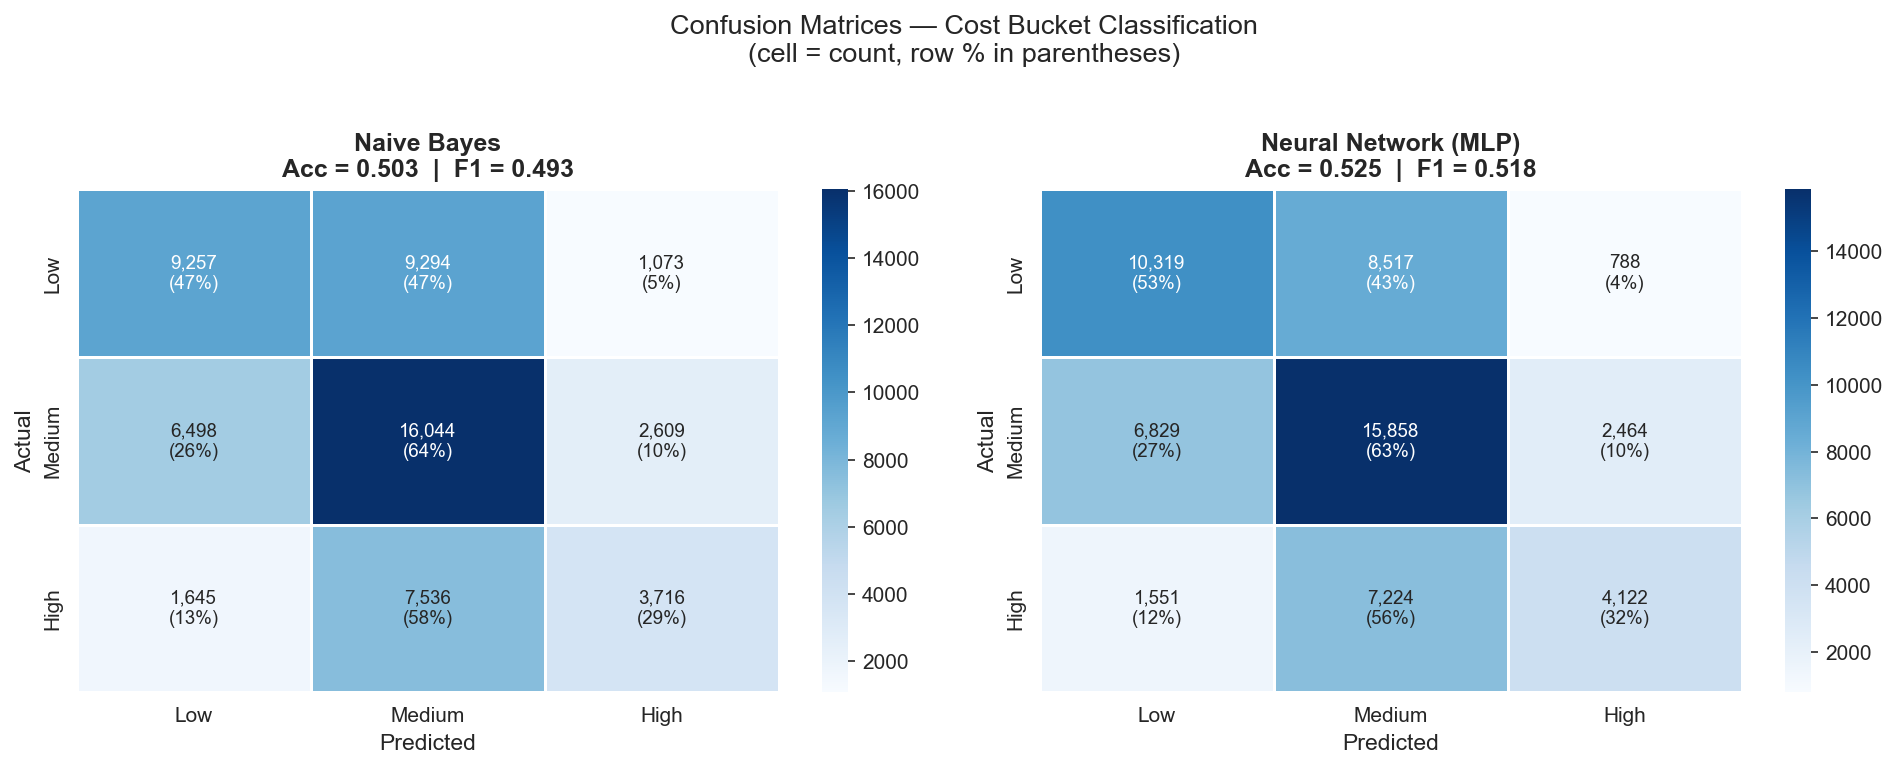
\includegraphics[width=0.9\textwidth]{fig_confusion_matrices.png}
    \caption{Confusion matrices for Naive Bayes and MLP (cell = count, row \%). Adjacent-bucket errors dominate; the MLP shows more balanced per-class recall.}
    \label{fig:confusion}
\end{figure}

\subsection{PCA Visualization and Unsupervised Validation}

Figure~\ref{fig:pca} shows a PCA projection of 3,000 papers reduced via Truncated SVD (50 components, explaining 12.5\% of variance) followed by PCA (2 components). K-Means with $k = 3$ achieves a cluster purity of \textbf{0.4363} versus a random-assignment baseline of 0.3333---a relative improvement of 30.9\%---confirming that cost-associated vocabulary forms emergent structure in TF-IDF space.

\begin{figure}[h]
    \centering
    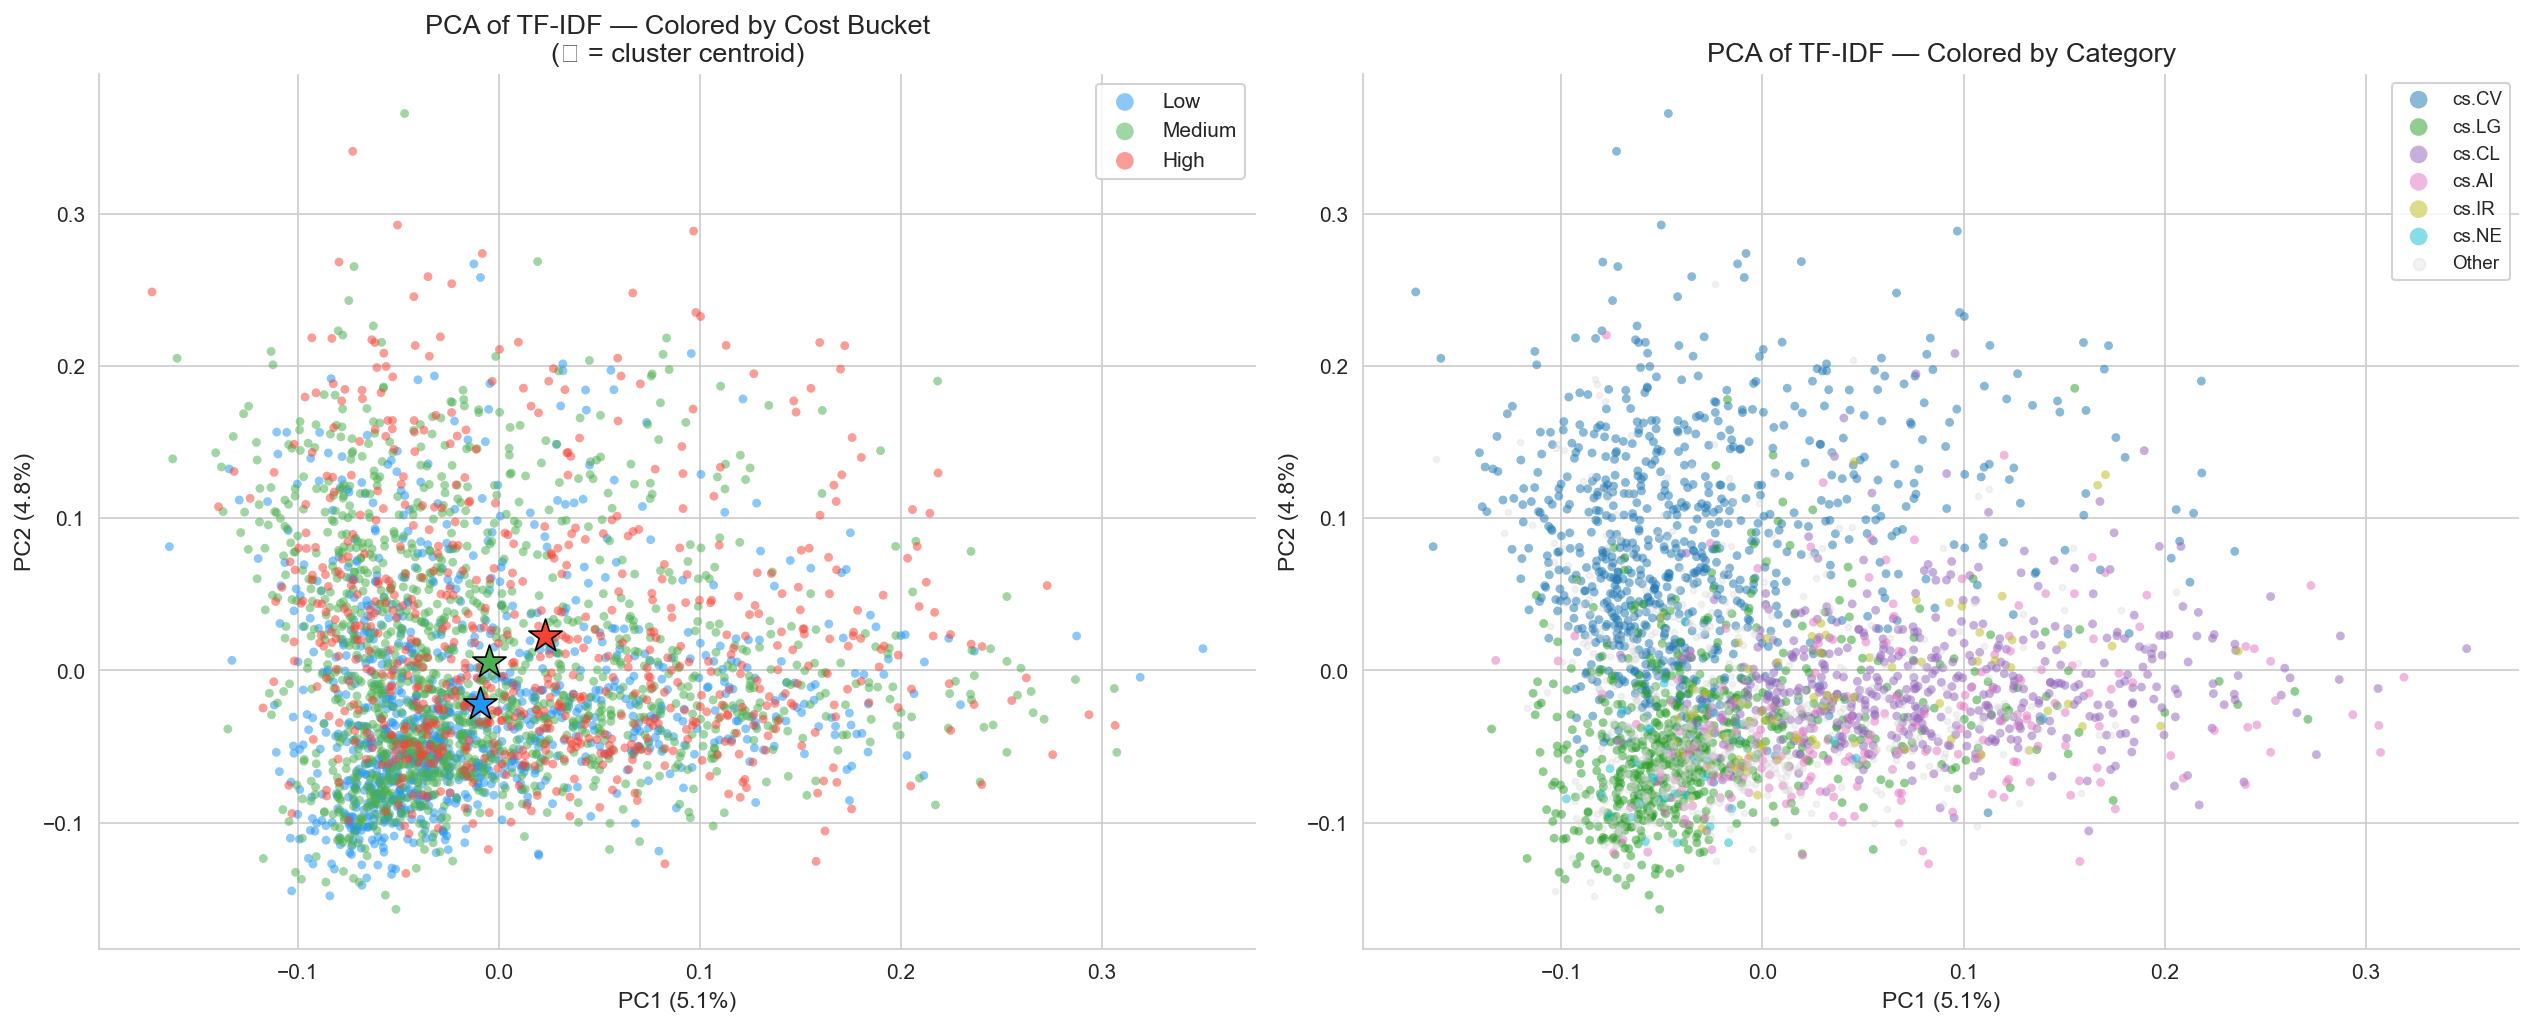
\includegraphics[width=\textwidth]{fig_pca_visualization.png}
    \caption{Left: PCA of TF-IDF features colored by cost bucket. Right: colored by ArXiv category. SVD explains 12.5\% of variance in 50 components. Partial separation by cost bucket confirms that title and abstract vocabulary carries cost signal.}
    \label{fig:pca}
\end{figure}

\subsection{L2 Regularization Ablation}

Table~\ref{tab:l2} tests four regularization strengths for LR. Results are identical across all $\lambda$ values, showing the model always collapses to the Medium majority class regardless of regularization. The near-zero weight norm ($\|\mathbf{w}\|_2 \approx 0.12$) suggests the gradient signal is simply too weak for 230K samples across 10K features --- LR never meaningfully learns from the data.

\begin{table}[h]
    \centering
    \caption{L2 regularization ablation for Logistic Regression OvR ($\eta = 0.01$, 500 iterations). Identical results across all $\lambda$ indicate majority-class collapse rather than genuine convergence.}
    \label{tab:l2}
    \begin{tabular}{cccc}
        \toprule
        $\lambda$ & Accuracy & Weighted F1 & $\|\mathbf{w}\|_2$ \\
        \midrule
        0.01 & 0.4361 & 0.2649 & 0.12 \\
        0.10 & 0.4361 & 0.2649 & 0.12 \\
        1.00 & 0.4361 & 0.2649 & 0.12 \\
        10.0 & 0.4361 & 0.2649 & 0.12 \\
        \bottomrule
    \end{tabular}
\end{table}

This is why the MLP (F1 = 0.5179) so clearly outperforms LR (F1 = 0.2649) --- its hidden layers can discover patterns in the data that a linear classifier simply cannot represent at this scale.

\subsection{LR Convergence}

Figure~\ref{fig:convergence} shows loss curves for all three OvR classifiers over 500 iterations. Training is stable --- the collapse to majority-class prediction is a model capacity problem, not a numerical one.

\begin{figure}[h]
    \centering
    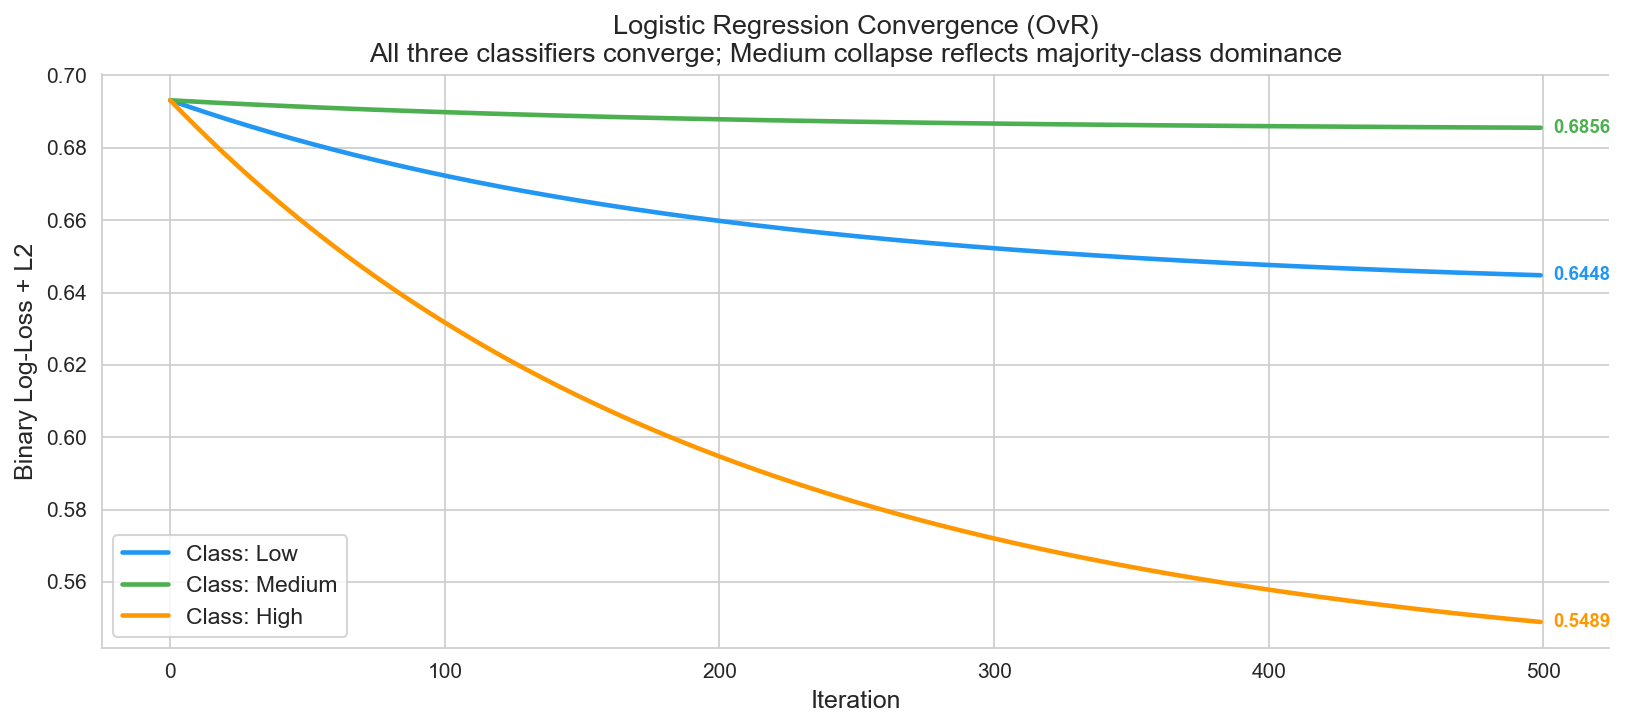
\includegraphics[width=0.85\textwidth]{fig_lr_convergence.png}
    \caption{Logistic Regression OvR convergence curves (500 iterations, $\eta = 0.01$, $\lambda = 10.0$). Loss decreases smoothly but the model converges to a degenerate majority-class solution, confirming the capacity limitation revealed in Table~\ref{tab:l2}.}
    \label{fig:convergence}
\end{figure}

\subsection{Temporal and Category Cost Analysis}

Table~\ref{tab:yearly} shows the estimated total human capital investment in AI research per year. The aggregate cost across all 288,368 papers is \textbf{\$11.6 billion} over the period. Full-year costs grew from \$2.57B in 2023 to \$4.54B in 2025 as ArXiv submission volume expanded significantly (2022 and 2026 are partial years and excluded from the growth comparison).

\begin{table}[h]
    \centering
    \caption{Estimated total human capital cost of AI research per year across all six ArXiv categories.}
    \label{tab:yearly}
    \begin{tabular}{ccrr}
        \toprule
        \textbf{Year} & \textbf{Papers} & \textbf{Total Cost} & \textbf{Mean per Paper} \\
        \midrule
        2022\textsuperscript{†} &   4,073 & \$152M  & \$37,306 \\
        2023 &  67,694 & \$2.56B & \$37,798 \\
        2024 &  87,862 & \$3.50B & \$39,886 \\
        2025 & 108,124 & \$4.53B & \$41,874 \\
        2026\textsuperscript{*} & 20,615 & \$861M & \$41,761 \\
        \midrule
        \textbf{Total} & \textbf{288,368} & \textbf{\$11.6B} & \textbf{\$40,239} \\
        \bottomrule
    \end{tabular}
    \\[4pt]\small\textsuperscript{†}Partial year (December 2022 only). \textsuperscript{*}Partial year (January--March 5, 2026).
\end{table}

Figure~\ref{fig:temporal} shows mean estimated cost by month (December 2022--February 2026; March 2026 excluded as a partial month of only 5 days), with the category panel restricted to full years 2023--2025 to avoid partial-year skew. Table~\ref{tab:categories} summarizes costs across all six ArXiv categories.

\begin{table}[h]
    \centering
    \caption{Estimated human capital cost per paper for all six ArXiv categories (all 288,368 papers).}
    \label{tab:categories}
    \begin{tabular}{lcccc}
        \toprule
        \textbf{Category} & \textbf{Papers} & \textbf{Mean Cost} & \textbf{Median Cost} & \textbf{Mean Authors} \\
        \midrule
        cs.CL (Computation \& Language) & 46,317 & \$43,992 & \$39,079 & 5.7 \\
        cs.CV (Computer Vision)         & 76,469 & \$43,008 & \$39,079 & 5.6 \\
        cs.AI (Artificial Intelligence) & 19,205 & \$42,537 & \$32,258 & 5.5 \\
        cs.IR (Information Retrieval)   &  7,132 & \$42,142 & \$39,079 & 5.4 \\
        cs.NE (Neural \& Evol.\ Comp.)  &  2,645 & \$31,780 & \$25,437 & 3.9 \\
        cs.LG (Machine Learning)        & 68,631 & \$36,150 & \$32,258 & 4.6 \\
        \bottomrule
    \end{tabular}
\end{table}

\begin{figure}[h]
    \centering
    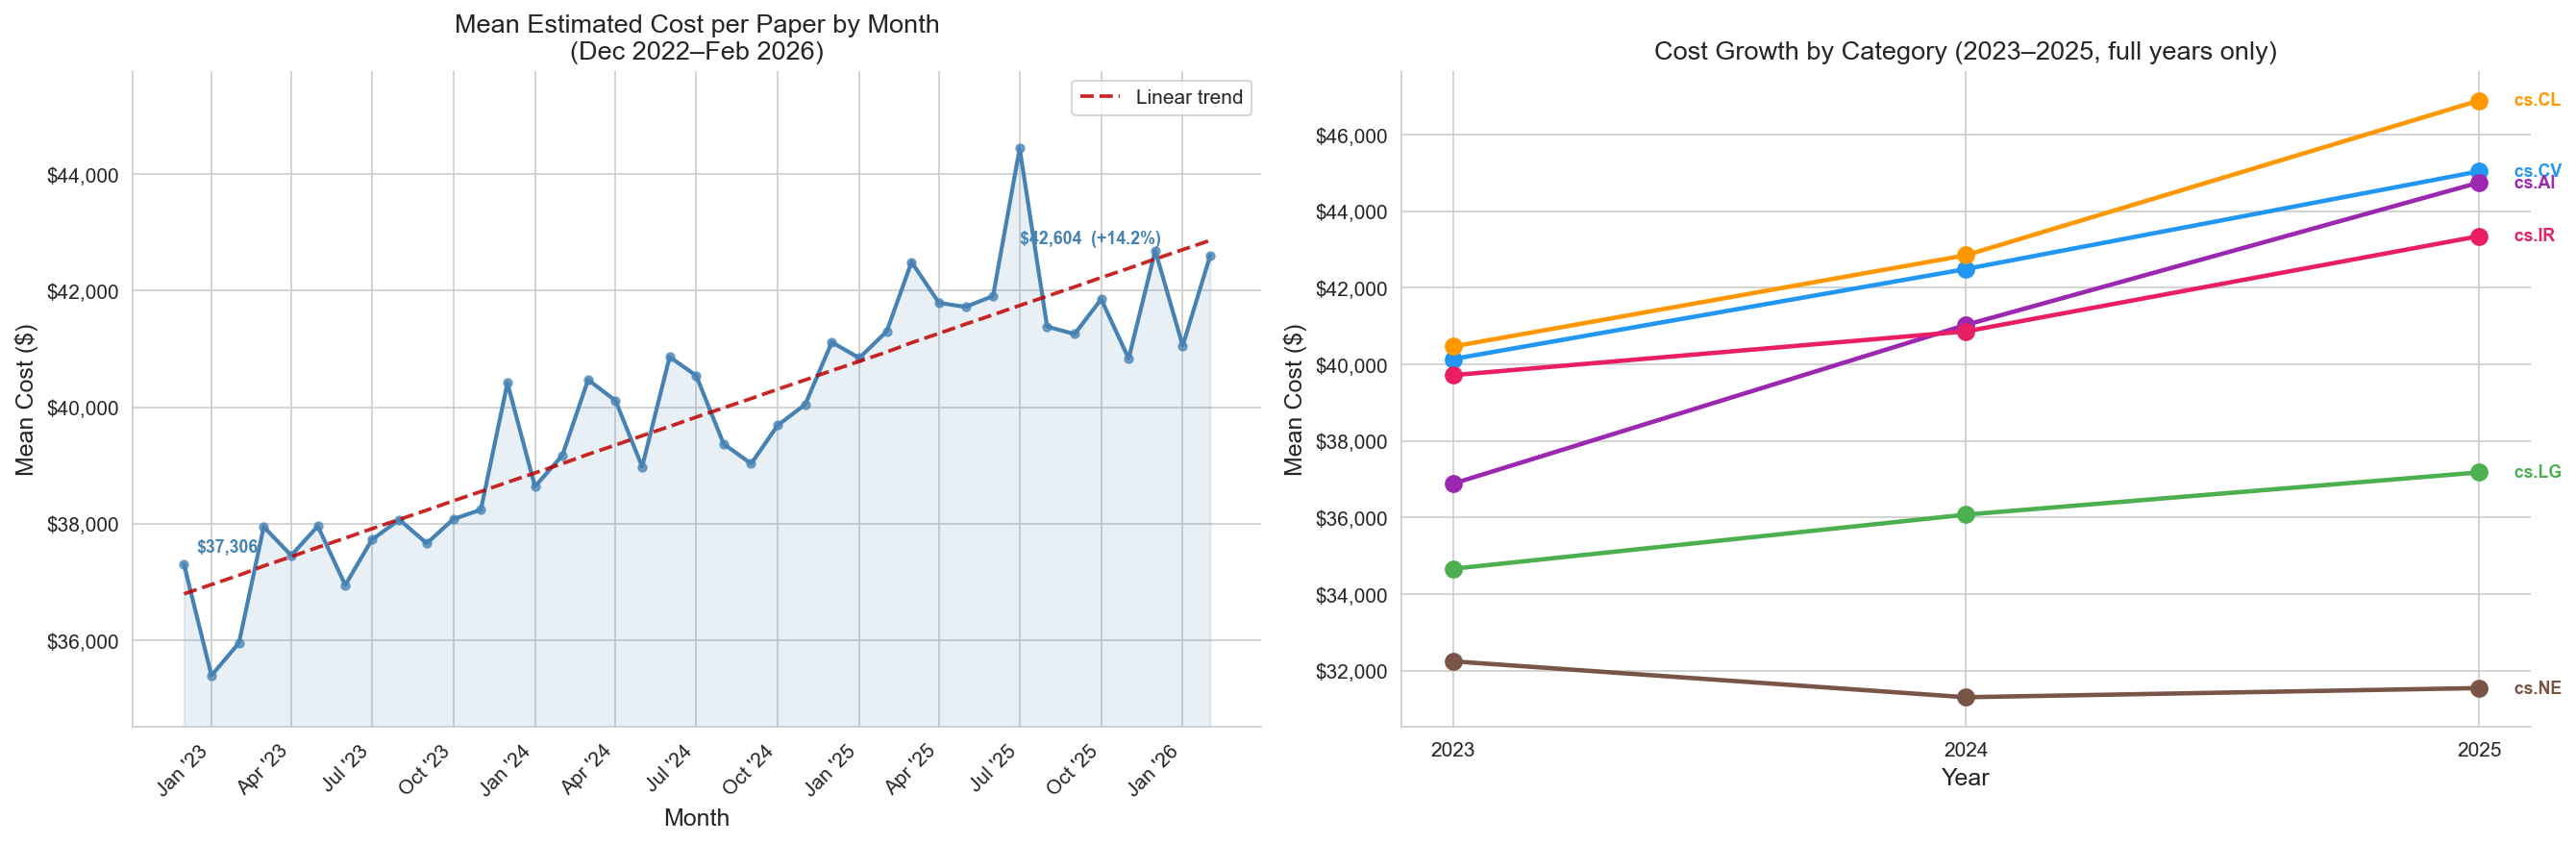
\includegraphics[width=\textwidth]{fig_temporal_analysis.png}
    \caption{Left: mean estimated cost per paper by month (December 2022--February 2026; March 2026 excluded as partial month). Right: mean cost by category for full years 2023--2025 only (partial years 2022 and 2026 excluded to avoid skew).}
    \label{fig:temporal}
\end{figure}

\section{Discussion}

\textbf{What does the NLP signal capture?}
The MLP reaches F1 = 0.5179 versus a 0.333 random baseline, which means the text genuinely carries some cost signal. Looking at the PCA plot, High-cost papers cluster around large-scale systems language while Low-cost papers lean toward theory vocabulary --- exactly what we'd expect if expensive papers tend to have bigger, more applied teams. That said, cost is really driven by who wrote the paper, not what it says. The NLP models are picking up on vocabulary as a proxy for team composition.

\textbf{Limitations.}
The biggest limitation is that every cost estimate comes from the same fixed salary priors. Two papers with identical team structures get identical cost estimates even if one has senior researchers from top institutions and the other has mostly undergrads. The model has no way to distinguish that. Real per-author salary data would make the labels much more meaningful.

\textbf{The cost growth trend} reflects both genuine salary growth in AI research roles and the trend toward larger author teams in recent papers---a structural change in how AI research is conducted.

\section{Conclusion}

This work, developed for 01:198:439 Introduction to Data Science~\cite{wang2026course}, demonstrates that human capital costs of AI research papers can be meaningfully estimated from authorship metadata, and that paper text carries moderate but real predictive signal for cost tier.

\textbf{Future Work.}
The most direct improvement is replacing the median salary priors with real compensation data — actual PhD stipends, postdoctoral salaries from public disclosures, or institutional grant and funding records. The current approach of manually entered medians is a reasonable starting point but remains susceptible to human error and cannot capture variation across institutions or countries. More precise cost labels would directly improve the NLP classification task.

Beyond data quality, a more expansive direction is extending this analysis across all of ArXiv rather than only CS subfields, to understand where AI research is heading at a broader scale. Three themes stand out as worth investigating in future iterations:

\textbf{Control.} Large language models are one component of what will likely become networks of interacting AI systems. As these systems grow in capability and become embedded across governments, economies, and infrastructure, fundamental questions of governance emerge: who controls them, whether they operate for public or private benefit, and how accountability is maintained when decision-making authority is diffuse across many interconnected systems.

\textbf{Management.} AI is already functioning as a productivity tool that reshapes how knowledge work is organized. The near-term question is what happens to the researchers and engineers building these systems once the engineering phase matures. A longitudinal analysis of labor patterns across all ArXiv disciplines — tracking which fields grow or shrink and at what rate — could provide early signals of structural shifts in the research workforce.

\textbf{Abundance.} The most speculative but arguably most consequential question is whether AI can be directed toward eliminating material scarcity. Existing governance structures have historically struggled to coordinate resources at scale; if sufficiently capable AI systems can transcend those coordination failures, they may represent a realistic path toward a world where foundational needs are reliably met for everyone. Whether that outcome is governed by public institutions, private entities, or something else entirely is perhaps the most important design question of the coming decades.

\clearpage
\bibliographystyle{plain}
\begin{thebibliography}{99}

\bibitem{mckinney2022}
McKinney, W. (2022).
\textit{Python for Data Analysis} (3rd ed.).
O'Reilly Media.
\url{https://wesmckinney.com/book/}
\textit{[Module 1 — Python, Pandas, NumPy: data loading and cost pipeline.]}

\bibitem{learningds2023}
Lau, S., Gonzalez, J., \& Nolan, D. (2023).
\textit{Learning Data Science}.
O'Reilly Media.
\url{https://learningds.org/}
\textit{[Module 2 — EDA, KDE, Text/Regex, Visualization: author distribution and cost analysis.]}

\bibitem{vanderplalas2023}
VanderPlas, J. (2023).
\textit{Python Data Science Handbook} (2nd ed.).
O'Reilly Media.
\url{https://jakevdp.github.io/PythonDataScienceHandbook/}
\textit{[Module 3 — SVD, PCA, Dimension Reduction: TF-IDF matrix, PCA/K-Means visualization.]}

\bibitem{princetondml}
Princeton COS 324 (2024).
\textit{Introduction to Machine Learning} (Course Notes).
Princeton University.
\url{https://princeton-introml.github.io/}
\textit{[Modules 4--5 — NB, LR, Gradient Descent, Regularization, Clustering, Neural Networks: all classifiers and K-Means.]}

\bibitem{haddii2024}
Haddii, U. (2024).
ArXiv AI Research Papers Dataset.
\textit{Kaggle}.
\url{https://www.kaggle.com/datasets/umerhaddii/arxiv-ai-research-papers-dataset}.
Licensed under CC BY 4.0.

\bibitem{wang2026course}
Wang, H. (2026).
\textit{01:198:439 Introduction to Data Science} (Course).
Rutgers University.
Modules: [1] Python/Pandas, [2] EDA/KDE/Visualization, [3] SVD/PCA/Dimension Reduction,
[4] NB/LR/Gradient Descent/Regularization/Clustering, [5] Deep Learning/Neural Networks.

\end{thebibliography}

\end{document}
